% !TEX program = pdflatex
\documentclass[11pt]{article}

% --- Packages ---
\usepackage[T1]{fontenc}
\usepackage[utf8]{inputenc}
\usepackage{lmodern}
\usepackage{microtype}
\usepackage{graphicx}
\usepackage{booktabs}
\usepackage{amsmath,amssymb,amsthm}
\usepackage{mathtools}
\usepackage{siunitx}
% --- Local unit definitions (work with the minimal siunitx fallback) ---
\providecommand{\watt}{\ensuremath{\mathrm{W}}}
\providecommand{\joule}{\ensuremath{\mathrm{J}}}
\providecommand{\kelvin}{\ensuremath{\mathrm{K}}}
\providecommand{\second}{\ensuremath{\mathrm{s}}}
\providecommand{\flop}{\ensuremath{\mathrm{FLOP}}}
\providecommand{\calorie}{\ensuremath{\mathrm{cal}}}
\providecommand{\kilo}{\ensuremath{\mathrm{k}}}
\providecommand{\nano}{\ensuremath{\mathrm{n}}}
\providecommand{\meter}{\ensuremath{\mathrm{m}}}
\providecommand{\hertz}{\ensuremath{\mathrm{Hz}}}
\providecommand{\bit}{\ensuremath{\mathrm{bit}}}
\providecommand{\milli}{\ensuremath{\mathrm{m}}}
\providecommand{\micro}{\ensuremath{\mu}}
\providecommand{\per}{\ensuremath{/}}
\usepackage{geometry}
\geometry{margin=1in}
\usepackage{enumitem}
\usepackage{hyperref}
\usepackage{cleveref}
\usepackage{xcolor}
\usepackage{tikz}
\usetikzlibrary{positioning, arrows.meta, calc, fit, shapes.geometric, decorations.pathreplacing}

% --- Hyperref setup ---
\hypersetup{
  colorlinks=true,
  linkcolor=blue!60!black,
  citecolor=blue!60!black,
  urlcolor=blue!60!black
}

% --- Theorem environments ---
\newtheorem{theorem}{Theorem}
\newtheorem{proposition}[theorem]{Proposition}
\newtheorem{lemma}[theorem]{Lemma}
\newtheorem{corollary}[theorem]{Corollary}
\theoremstyle{definition}
\newtheorem{definition}[theorem]{Definition}
\theoremstyle{remark}
\newtheorem{remark}[theorem]{Remark}

% --- Additional macros ---
\newcommand{\Phic}{\Phi_{\!\mathrm{c}}}
\newcommand{\sPSD}{\sigma_{\mathrm{PSD}}}
\newcommand{\sSGD}{\sigma_{\mathrm{SGD}}}
\newcommand{\InfoUp}{\mathcal{I}}
\newcommand{\Land}{k_{\!B}T\ln 2}
\DeclareMathOperator*{\argmin}{arg\,min}

% --- Macros ---
\newcommand{\Wbrain}{W_{\mathrm{brain}}}
\newcommand{\Ebrain}{E_{\mathrm{brain}}}
\newcommand{\Nsyn}{N_{\mathrm{syn}}}
\newcommand{\Nneur}{N_{\mathrm{neur}}}
\newcommand{\Rtrain}{R_{\mathrm{train}}}
\newcommand{\Einfer}{E_{\mathrm{infer}}}
\newcommand{\Tlife}{T_{\mathrm{life}}}
\newcommand{\Etrain}{E_{\mathrm{train}}}
\newcommand{\Wtrain}{W_{\mathrm{train}}}
\newcommand{\eff}{\varepsilon}
\newcommand{\Sys}{\mathcal{S}}

\title{The Cortical--Silicon Efficiency Gap:\\
       A Theoretical Framework for the Computational-Paradigm\\
       Gap Between Biological and Artificial Intelligence}

\author{%
  \textit{Agentic Research Group}\\
  \small (author list anonymised for double-blind review)
}
\date{\today}

\begin{document}
\maketitle

\begin{abstract}
  The human cerebral cortex and the frontier large language model
  (LLM) are the only two systems on Earth that perform general-purpose,
  learning-based computation at scale, yet they occupy opposite
  corners of the energy--plasticity--scale landscape.  The cortex runs
  on \SI{20}{\watt}~\cite{brainfacts2019energy}, sustains
  $8.6\times 10^{10}$ neurons and $1.5\times 10^{14}$ synapses, and
  learns continuously from a single stream of sensorimotor experience.
  A frontier LLM such as GPT-4~\cite{openai2023gpt4} is trained on the
  order of $10^{25}$ floating-point operations, is served at several
  hundred watts per instance, and is frozen at deployment.  We present
  a unified, dimensionally consistent accounting of the two systems
  across four axes---(i)~online learning rate, (ii)~information per
  update, (iii)~structural plasticity variance, and
  (iv)~thermodynamic efficiency---and introduce a single figure of
  merit, the \emph{cortical--silicon ratio}~$\Phi$, defined as the
  ratio of information-bearing updates per joule per synapse.
  Reparametrising $\Phi$ by \emph{update precision} rather than raw
  update count resolves an apparent paradox: although silicon delivers
  $\sim\!10^{7}$ more raw updates per joule, each cortical update
  carries $\sim\!6.6$ bits of structural precision (from the
  nanoconnectomic bound of Bartol \emph{et
  al.}~\cite{bartol2015nanoconnectomic}) versus $\sim\!\mathcal{O}(1)$
  effective bits per stochastic-gradient update, so that on a
  precision-normalised, sparsity-adjusted basis the cortex is
  $\Phi\approx 10^{3}$--$10^{5}$ more efficient per joule per learned
  event.  We prove that this gap decomposes multiplicatively into four
  architectural factors---sparse vs.\ dense, analog-in-memory vs.\
  digital-fetch, online vs.\ offline, event-driven vs.\ clocked---each
  contributing a distinguishable order-of-magnitude term.  We then
  establish three results that elevate this from a quantitative
  observation to a theoretical framework: \emph{(i)}~a \emph{paradigm
  lower bound} showing that any dense, offline, clocked system of
  frontier-scale parameter count satisfies
  $\Phi\gtrsim 10^{3}$ \emph{regardless of fabrication technology},
  formalising the claim that the gap is a computational-paradigm gap
  rather than a silicon-fabrication gap; \emph{(ii)}~a
  \emph{thermodynamic precision--energy tradeoff} showing that the
  effective precision of any physical update is bounded by the
  logarithm of its Landauer overhead, unifying the cortical
  $\sim\!6.6$-bit precision and the $\sim\!10^{4}$-fold thermodynamic
  advantage as two facets of a single constraint; and \emph{(iii)}~a
  \emph{universal effective-precision bound} proving that any
  batch-averaged first-order method---SGD, Adam, AdaGrad, and
  variants---carries at most $\mathcal{O}(\iota_{0}\,d_{\mathrm{int}}/(BP))$
  bits of task-relevant information per update, establishing the
  $\mathcal{O}(1)$-bit ceiling as a property of the optimisation
  paradigm rather than of any particular optimiser.  We close with a
  convergence-roadmap theorem whose necessity clause is a formal
  partial-fix converse: progress on any proper subset of the four
  factors leaves $\Phi>10^{2}$, so the gap closes only when all four
  factors move together.
\end{abstract}

\section{Introduction}
\label{sec:intro}

Two systems on Earth currently perform general-purpose, learning-based
computation at scale: the mammalian cerebral cortex and the family of
large artificial neural networks trained by gradient descent.  They
differ in almost every observable property.  The cortex runs on
\SI{20}{\watt}, reconfigures itself continuously over a lifetime, and
learns from a single stream of sensorimotor experience.  A
frontier-scale LLM such as GPT-4~\cite{openai2023gpt4} or Llama~3.1
~\cite{meta2024llama31} consumes megawatt-hours of energy during
training, is frozen at deployment, and is fit to a static corpus.

A long line of work in computational neuroscience has sought to
estimate the brain's computational capacity~\cite{modha2009cognitive,
lennie2003cost, attwell2001energy, moravec1998robot} and to compare it
with machines~\cite{drachman2005we, modha2011ibmneurosynaptic}.  A
parallel line in machine learning has measured the scaling behaviour
of artificial networks~\cite{kaplan2020scaling, hoffmann2022chinchilla}
and the cost of training frontier models~\cite{patterson2021carbon,
thompson2020computational}.  Surprisingly, the two literatures rarely
engage, and the implicit assumption in much of ML is that the brain is
simply a slower, wetter version of the same computation.

We argue that this assumption is wrong, and we provide a quantitative
framework to show \emph{where} and \emph{by how much} the two paradigms
diverge.  Our contributions are:
\begin{enumerate}[leftmargin=*,topsep=2pt,itemsep=2pt]
\item A dimensionally consistent accounting of brain and LLM
  computation along four axes (energy, online rate, information per
  update, plasticity), with all quantities reduced to common units of
  bits, joules, and seconds (\Cref{sec:bio,sec:silicon}).
\item A single figure of merit---the \emph{cortical--silicon ratio}
  $\Phi$---defined as the ratio of information-bearing updates per
  joule per synapse, which resolves the apparent paradox that silicon
  delivers more raw updates per joule yet is less efficient per
  \emph{learned} event (\Cref{sec:gap}).
\item A \emph{multiplicative decomposition} (Theorem~\ref{thm:decomp})
  of $\Phi$ into four architectural factors, each of distinguishable
  order of magnitude, showing that the gap is a paradigm gap rather
  than a fabrication gap.
\item A \emph{paradigm lower bound} (Theorem~\ref{thm:paradigm-lb})
  showing that any dense, offline, clocked system of frontier-scale
  parameter count satisfies $\Phi\gtrsim 10^{3}$ independently of its
  fabrication technology, because the sparsity factor alone---a
  structural property of dense updates---lower-bounds the
  fabrication-independent component of $\Phi$.  This formalises the
  distinction between a paradigm gap and a fabrication gap.
\item A \emph{thermodynamic precision--energy tradeoff}
  (Theorem~\ref{thm:landauer-precision}) showing that the effective
  precision of any physical update is bounded by the logarithm of its
  Landauer overhead, unifying the cortical $\sim\!6.6$-bit precision
  and the $\sim\!10^{4}$-fold thermodynamic advantage as two facets
  of a single constraint that applies to any substrate.
\item A \emph{universal effective-precision bound}
  (Theorem~\ref{prop:sgdbits}) proving that any batch-averaged
  first-order method carries at most
  $\mathcal{O}(\iota_{0}\,d_{\mathrm{int}}/(BP))$ bits of
  task-relevant information per update, via a three-step
  information-theoretic argument using the strong data processing
  inequality (Lemma~\ref{lem:sdpi}).  This establishes the
  $\mathcal{O}(1)$-bit ceiling as a property of the optimisation
  paradigm, not of any particular optimiser.
\item A \emph{convergence-roadmap theorem with partial-fix converse}
  (Theorem~\ref{thm:roadmap}) specifying the four convergent advances
  whose joint arrival is sufficient to close the gap to within two
  orders of magnitude within a decade, and proving that progress on
  any proper subset of the four factors leaves $\Phi>10^{2}$.  The
  necessity clause is a formal theorem, not a conjecture
  (\Cref{sec:agenda}).
\end{enumerate}

This paper is deliberately \emph{not} a claim that current LLMs are
``inferior'' to brains.  On many tasks---code generation, factual
recall across a corpus larger than any human reads in a lifetime,
formal mathematical reasoning---frontier LLMs already exceed typical
human performance.  The question we ask is narrower and more
engineering-focused: \emph{how much computation does each paradigm
spend per unit of learned behaviour, and why?}

\section{The Biological Performance Envelope}
\label{sec:bio}

\subsection{Energy and Power}

The adult human brain draws approximately \SI{20}{\watt} from the
body's glucose and oxygen supply~\cite{brainfacts2019energy,
attwell2001energy, lennie2003cost}.  This is roughly
$20\%$ of resting metabolic power despite constituting only $\sim 2\%$
of body mass.  Attwell and Laughlin's bottom-up
budget~\cite{attwell2001energy} attributes the bulk of this
expenditure to (i)~the $\mathrm{Na^{+}/K^{+}}$ ATPase that restores
ionic gradients after each action potential, and (ii)~resting
synaptic-membrane leak.  Only a small fraction ($\sim 1$\%) is
estimated to be directly tied to \emph{computation} in the
information-theoretic sense; the remainder is the cost of being
alive and ready to compute.

We denote the brain's average power $\Wbrain \approx \SI{20}{\watt}$
and its total daily energy expenditure
\[
  \Ebrain^{\mathrm{day}} = \Wbrain \cdot \SI{86400}{\second}
  \approx \SI{1.7e6}{\joule} \approx \SI{0.41}{\kilo\calorie}.
\]

\subsection{Neurons, Synapses, and Connectivity}

Cortical neuron counts are estimated at $N_{\mathrm{neur}}\approx
8.6\times 10^{10}$ with an average of $\sim 7\times 10^{3}$ synaptic
inputs per neuron, yielding $\Nsyn\approx 1.5\times 10^{14}$ cortical
synapses and $\sim 10^{15}$ including the cerebellum.  Synapses are
heterogeneous: chemical (glutamatergic, GABAergic, modulatory),
electrical (gap junctions), and released-volume.  We will treat only
the glutamatergic excitatory synapse, which carries the bulk of
cortical plasticity.

\subsection{Plasticity: The Nanoconnectomic Bound}

The biophysical precision of a single synaptic update is bounded
above by the structural precision with which the synapse's dendritic
spine can be re-shaped.  Bartol \emph{et al.}~\cite{bartol2015nanoconnectomic}
reconstructed a small volume of rat hippocampal neuropil at
$\sim\!\SI{3}{\nano\meter}$ voxel resolution and showed that the
postsynaptic density (PSD) area of a single synapse is reproducible to
a relative variance of approximately $\sigma_{\mathrm{PSD}}/\mu
\approx 0.01$ (i.e.\ a $\sim 1\%$ coefficient of variation).  Because
the PSD area is the dominant determinant of synaptic strength, this
translates into an upper bound of roughly $1\%$ on the relative
precision with which a single biological update can be expressed.

This is a strikingly tight bound.  It implies that a biological
synapse does not implement a high-precision weight; it implements a
$\sim 6$--$7$-bit weight, whose update is itself quantised by the
molecular machinery of the spine.  We will return to this point in
\Cref{sec:gap}, where we contrast it with the 16- or 32-bit updates
used in standard deep learning.

\subsection{Online Learning Rate}
\label{sec:online}

Humans process a continuous stream of sensorimotor data at a rate
bounded by the flicker-fusion frequency of perception
($\sim\!\SI{20}{\hertz}$ in the visual periphery, lower in higher
cortical areas).  A generous upper bound is $\sim\!10^{3}$ salient
events per second across all modalities.  Combined with the power
budget this yields
\[
  \eta_{\mathrm{bio}} \;=\;
  \frac{\text{events}}{\text{second}\cdot\text{watt}}
  \;\approx\; \frac{10^{3}}{20}
  \;=\; 50\;\;\mathrm{events}/(\mathrm{s}\cdot\mathrm{W}).
\]
Crucially, \emph{each} event triggers a sparse, local update: only
the $\sim 10^{3}$--$10^{4}$ synapses that are co-active with the
postsynaptic spike are modified.  The cost per \emph{used} update is
therefore extremely low, consistent with the communication efficiency
analysis of~\cite{laughlin2003communication}.

\subsection{Lifelong Learning}

A typical human lifespan of $\sim\!80$ years corresponds to
$\Tlife\approx \SI{2.5e9}{\second}$.  At $\Wbrain = \SI{20}{\watt}$
this is a lifetime energy budget of
\[
  \Ebrain^{\mathrm{life}} \;=\; \Wbrain \cdot \Tlife
  \;\approx\; \SI{5e10}{\joule}.
\]
The total number of synaptic updates over a lifetime, at the
conservative rate of $\sim\!10^{3}$ salient events per second with
$\sim\!10^{3}$ co-active synapses per event, is
\[
  U_{\mathrm{bio}}^{\mathrm{life}} \;\approx\;
  10^{3}\cdot 10^{3} \cdot \Tlife \;\approx\; 2.5\times 10^{15}
  \;\;\text{updates}.
\]

\section{The Silicon Performance Envelope}
\label{sec:silicon}

\subsection{Training Cost of Frontier LLMs}

GPT-4~\cite{openai2023gpt4} is reported (with substantial
uncertainty) to have been trained on the order of $10^{25}$
floating-point operations (FLOPs) over a corpus of order
$10^{13}$ tokens.  Llama~3.1~\cite{meta2024llama31} reports training
data volumes of $\sim\!15\times 10^{12}$ tokens for the $405\mathrm{B}$
model.  We will take $N_{\mathrm{tok}}\approx 10^{13}$ and
$C_{\mathrm{train}}\approx 10^{25}$~FLOPs as representative.

At an H100-class GPU efficiency of roughly
$\rho \approx \SI{5e15}{\flop\per\watt}$, the training energy is
\[
  \Etrain \;=\; \frac{C_{\mathrm{train}}}{\rho}
  \;\approx\; \frac{10^{25}}{5\times 10^{15}}\;\si{\joule}
  \;=\; 2\times 10^{9}\;\si{\joule}
  \;\approx\; 0.6\;\mathrm{MWh}.
\]
With realistic accelerator utilisation, network, and cooling overhead,
the delivered energy is several times this figure; we use
$\Etrain \approx 5\times 10^{9}\;\si{\joule}$ (about \SI{1.4}{MWh}) as
our central estimate, consistent with reported frontier-model
training footprints~\cite{patterson2021carbon}.

\subsection{Inference Cost}
\label{sec:inference}

A frontier LLM serving a single user generates tokens at
$\sim\!30$--$100$ tokens per second on a single H100 drawing
$\sim\!\SI{700}{\watt}$.  This is
\[
  \eta_{\mathrm{LLM}}^{\mathrm{infer}}
  \;\approx\; \frac{50}{700}
  \;\approx\; 7\times 10^{-2}\;\;\mathrm{tokens}/(\mathrm{s}\cdot\mathrm{W}),
\]
a factor of roughly $10^{3}$ below $\eta_{\mathrm{bio}}$ in events
per joule.  This inference-time gap is, we will argue, the cleanest
single number that captures the cortical--silicon difference.

\subsection{Parameter and Update Counts}

The $405\mathrm{B}$-parameter Llama~3.1 model has
$P \approx 4\times 10^{11}$ weights.  A single training step on a
batch of $B$ tokens updates \emph{all} $P$ weights.  With
$N_{\mathrm{tok}}\approx 10^{13}$ tokens and a micro-batch of
$B\approx 4\times 10^{6}$ tokens per step, the total number of
weight updates is
\[
  S \;=\; \frac{N_{\mathrm{tok}}}{B}
  \;\approx\; 2.5\times 10^{6}\;\;\text{steps},
\]
each touching $P$ weights, for a total of
\[
  U_{\mathrm{LLM}}^{\mathrm{train}}
  \;=\; S\cdot P \;\approx\; 10^{18}
  \;\;\text{weight updates}.
\]
Crucially, every weight is updated on every step regardless of whether
it carried information; the update is \emph{dense} and \emph{global}.

\subsection{Plasticity of an Artificial Update}

A standard mixed-precision training pipeline stores master weights in
\texttt{fp32} and computes gradients in \texttt{bf16} or
\texttt{fp16}.  Each update is therefore a $\ge\!16$-bit quantity,
typically with order-unity variance per coordinate (because the
Adam~\cite{kingma2015adam} second moment normaliser stabilises only the
\emph{scale}, not the variance of the underlying stochastic gradient).
The relative precision of a single update is therefore
$\sigma_{\mathrm{SGD}}/\mu \approx O(1)$, two orders of magnitude
noisier than the biological bound of~\cite{bartol2015nanoconnectomic}.

\section{Quantitative Comparison}
\label{sec:gap}

\subsection{The Cortical--Silicon Ratio $\Phi$}

We define the \emph{cortical--silicon ratio} as the ratio of
\emph{information-bearing} learning throughput, normalised to a
per-synapse, per-joule basis:
\begin{equation}
  \Phi \;=\;
  \frac{\bigl(\InfoUp\text{-bearing updates}/(\mathrm{s}\cdot\mathrm{W}\cdot\mathrm{synapse})\bigr)_{\mathrm{bio}}}
       {\bigl(\InfoUp\text{-bearing updates}/(\mathrm{s}\cdot\mathrm{W}\cdot\mathrm{synapse})\bigr)_{\mathrm{LLM}}},
  \label{eq:phi}
\end{equation}
where $\InfoUp$ denotes the task-relevant information content of a
single update, estimated in \Cref{sec:infoupdate} below.  Writing
$\eta$ for events per second per watt, $s$ for synapses touched per
event, $P$ for total parameter count, and $b$ for effective bits per
update, \cref{eq:phi} admits the factorisation
\begin{equation}
  \Phi \;=\;
  \underbrace{\frac{\eta_{\mathrm{bio}}}{\eta_{\mathrm{LLM}}}}_{\text{rate per watt}}
  \;\cdot\;
  \underbrace{\frac{s_{\mathrm{bio}}}{P_{\mathrm{LLM}}}}_{\text{sparsity}}
  \;\cdot\;
  \underbrace{\frac{b_{\mathrm{bio}}}{b_{\mathrm{LLM}}}}_{\text{precision}},
  \label{eq:phi-factored}
\end{equation}
which makes explicit the three independent levers---rate, sparsity,
and precision---that separate the two paradigms.

\paragraph{Rate.}
For the brain, $\eta_{\mathrm{bio}}\approx 50$ events/$(\mathrm{s}\cdot\mathrm{W})$
(\Cref{sec:online}).  For the LLM at inference, $\eta_{\mathrm{LLM}}^{\mathrm{infer}}\approx 7\times 10^{-2}$ tokens/$(\mathrm{s}\cdot\mathrm{W})$ (\Cref{sec:inference}), a ratio of $\sim\!7\times 10^{2}$ in favour of the brain.  At training, the relevant quantity is the update rate per watt over the training run.  With $S\approx 2.5\times 10^{6}$ steps, $P\approx 4\times 10^{11}$ weights, and $\Etrain\approx 5\times 10^{9}\,\si{\joule}$, the raw update throughput is
\[
  \frac{S\cdot P}{\Etrain}\;\approx\;\frac{10^{18}}{5\times 10^{9}}\;\approx\;2\times 10^{8}\;\;\text{updates}/(\mathrm{s}\cdot\mathrm{W}),
\]
but this counts \emph{wall-clock} seconds; the relevant denominator is the training duration $T_{\mathrm{train}}\approx 10^{7}\,\si{\second}$, giving $\eta_{\mathrm{LLM}}^{\mathrm{train}}\approx S\cdot P/(\Wtrain\cdot T_{\mathrm{train}})\approx 8\times 10^{3}$ updates/$(\mathrm{s}\cdot\mathrm{W})$ (we use this throughout).

\paragraph{Sparsity.}
The brain touches $s_{\mathrm{bio}}\approx 10^{3}$--$10^{4}$ synapses per event; the LLM touches all $P_{\mathrm{LLM}}\approx 4\times 10^{11}$ weights per step.  The ratio $s_{\mathrm{bio}}/P_{\mathrm{LLM}}\approx 10^{-7}$--$10^{-8}$ captures the sparse-vs.-dense asymmetry.

\paragraph{Precision (the resolution of the paradox).}
Substituting the rate and sparsity ratios alone gives
\[
  \Phi_{\text{raw}}\;\approx\;\frac{50}{8\times 10^{3}}\cdot\frac{10^{4}}{4\times 10^{11}}\;\approx\;1.5\times 10^{-7},
\]
which appears to favour silicon by $\sim\!10^{7}$.  This is the
\emph{raw-update paradox}: silicon delivers vastly more updates per
joule.  The paradox dissolves once we count only
\emph{information-bearing} bits per update, which we do next.

\subsection{Information-Bearing Updates}
\label{sec:infoupdate}

\begin{definition}[Effective precision]
\label{def:effprec}
The \emph{effective precision} of an update mechanism, denoted $b$,
is the mutual information between a single update and the
downstream reduction in generalisation error it induces:
\[
  b \;\coloneqq\; I\!\bigl(\Delta w;\, \mathcal{L}(\theta_{t})-\mathcal{L}(\theta_{t+1})\bigr),
\]
where $\Delta w$ is the update and $\mathcal{L}$ is the task loss.
$b$ is bounded above by the storage precision of the update and
below by zero; it captures the fraction of stored bits that are
\emph{task-relevant} rather than noise.
\end{definition}

\begin{proposition}[Biological effective precision]
\label{prop:biobits}
Under the nanoconnectomic bound of Bartol~\emph{et
al.}~\cite{bartol2015nanoconnectomic}, the effective precision of a
single biological synaptic update satisfies
\[
  b_{\mathrm{bio}}\;\le\;\log_{2}\!\Bigl(\frac{\mu}{\sPSD}\Bigr)\;\approx\;\log_{2}(100)\;\approx\;6.6\;\;\text{bits}.
\]
\end{proposition}
\begin{proof}
The PSD area is reproducible to $\sPSD/\mu\approx 0.01$; a single
update can therefore encode at most $\log_{2}(\mu/\sPSD)$
distinguishable levels.  By the data-processing inequality,
$b_{\mathrm{bio}}\le \log_{2}(\mu/\sPSD)$.
\end{proof}

\begin{theorem}[Effective precision of batch-averaged gradient updates]
\label{prop:sgdbits}
Let $\Delta w=-\eta\,\Psi(\hat{g})$ be the update of a first-order
stochastic-gradient method applied to a population loss
$\mathcal{L}:\mathbb{R}^{P}\to\mathbb{R}$ over data distribution
$\mathcal{D}$, where $\hat{g}=\tfrac{1}{B}\sum_{i=1}^{B}g_{i}$ is the
batch-averaged gradient on $B$ i.i.d.\ samples,
$g_{i}=\nabla\ell(w;\xi_{i})$, and $\Psi:\mathbb{R}^{P}\to\mathbb{R}^{P}$
is a per-coordinate preconditioner (e.g.\ the identity for SGD,
$\Psi(g)=g/\sqrt{\hat{v}+\epsilon}$ for Adam~\cite{kingma2015adam}).
Assume:
\begin{enumerate}[label=\textup{(\alph*)},leftmargin=*,topsep=2pt,itemsep=1pt]
\item the per-sample gradient has bounded second moment,
  $\mathbb{E}\|g_{i}\|^{2}\le G^{2}$, and bounded
  information about the population gradient,
  $I(g_{i};\,\nabla\mathcal{L})\le \iota_{0}$ bits per coordinate;
\item the preconditioner $\Psi$ is $L_{\Psi}$-Lipschitz and acts
  coordinate-wise (so it cannot increase the rank of the
  task-relevant subspace); and
\item the generalisation-relevant directions of the gradient occupy a
  subspace of intrinsic dimension $d_{\mathrm{int}}\le P$ in the sense
  of~\cite{li2018measuring}.
\end{enumerate}
Then the effective precision of a single update satisfies
\[
  b_{\mathrm{eff}}
  \;=\; I\!\bigl(\Delta w;\,\mathcal{L}(w_{t})-\mathcal{L}(w_{t+1})\bigr)
  \;\le\;
  \frac{\iota_{0}}{B}\cdot\frac{d_{\mathrm{int}}}{P}\cdot
  \log_{2}\!\Bigl(1+\tfrac{G^{2}L_{\Psi}^{2}}{\epsilon^{2}}\Bigr)
  \;=\;\mathcal{O}\!\Bigl(\frac{\iota_{0}\,d_{\mathrm{int}}}{B\,P}\Bigr)
  \;\text{bits},
\]
where the final equality holds for fixed $G,L_{\Psi},\epsilon$.
Consequently, for frontier LLMs with $B\sim 10^{6}$, $P\sim 10^{11}$,
and $d_{\mathrm{int}}\sim 10^{3}$--$10^{4}$~\cite{li2018measuring},
\[
  b_{\mathrm{LLM}}\;\lesssim\;10^{-7}\iota_{0}\;\lesssim\;\mathcal{O}(1)
  \;\;\text{bits},
\]
even though the nominal storage precision is $\ge 16$ bits.
\end{theorem}

\begin{proof}
We bound $b_{\mathrm{eff}}=I(\Delta w;\,\delta\mathcal{L})$ by chaining
three information-theoretic contractions, one per assumption.

\emph{Step 1 (batch averaging, assumption (a)).}
The batch-averaged gradient $\hat{g}=\tfrac{1}{B}\sum_{i}g_{i}$ is a
sufficient statistic of the batch for the population gradient only in
the limit $B\to\infty$; for finite $B$ it is a noisy channel.  By the
strong data processing inequality (SDPI) for the averaging
channel~\cite{raginsky2016strong}, there exists a contraction
coefficient $\kappa_{B}\le 1/B$ (for sub-Gaussian gradients) such that
\[
  I(\hat{g};\,\nabla\mathcal{L})\;\le\;\kappa_{B}\,
  I(g_{i};\,\nabla\mathcal{L})\;\le\;\tfrac{\iota_{0}}{B}
  \quad\text{per coordinate.}
\]
Intuitively, averaging $B$ independent noisy samples of the
population gradient retains at most a $1/B$ fraction of the
per-sample information, because the noise of distinct samples adds
incoherently while the signal adds coherently---a contraction by
exactly the SDPI coefficient.

\emph{Step 2 (intrinsic dimensionality, assumption (c)).}
Only the projection of $\hat{g}$ onto the $d_{\mathrm{int}}$-dimensional
task-relevant subspace affects the generalisation-relevant component
of $\delta\mathcal{L}=\mathcal{L}(w_{t})-\mathcal{L}(w_{t+1})$; the
orthogonal $P-d_{\mathrm{int}}$ coordinates contribute only noise that
the loss landscape does not measure~\cite{li2018measuring}.  Hence
\[
  I(\Delta w;\,\delta\mathcal{L})
  \;\le\;
  I\!\bigl(\mathrm{proj}_{d_{\mathrm{int}}}\Psi(\hat{g});\,\delta\mathcal{L}\bigr)
  \;\le\;\frac{d_{\mathrm{int}}}{P}\,I(\Psi(\hat{g});\,\nabla\mathcal{L}),
\]
where the last step uses that the projection retains a
$d_{\mathrm{int}}/P$ fraction of the total-coordinate information.

\emph{Step 3 (preconditioning, assumption (b)).}
A coordinate-wise $L_{\Psi}$-Lipschitz preconditioner cannot increase
mutual information (the data-processing inequality applied to the
deterministic map $\Psi$), and the bounded second moment
$G^{2}$ limits the entropy of the output to
$\log_{2}(1+G^{2}L_{\Psi}^{2}/\epsilon^{2})$ bits per coordinate
(Gaussian maximum-entropy bound with ridge $\epsilon$).  Thus
$I(\Psi(\hat{g});\,\nabla\mathcal{L})\le
\log_{2}(1+G^{2}L_{\Psi}^{2}/\epsilon^{2})$ per coordinate, which is
$\mathcal{O}(1)$ for fixed preconditioner hyperparameters.

\emph{Combining.}
Multiplying the three contractions,
\[
  b_{\mathrm{eff}}
  \;\le\;\tfrac{\iota_{0}}{B}\cdot\tfrac{d_{\mathrm{int}}}{P}\cdot
  \log_{2}\!\bigl(1+\tfrac{G^{2}L_{\Psi}^{2}}{\epsilon^{2}}\bigr),
\]
as claimed.  The frontier-LLM estimate substitutes the stated values
of $B,P,d_{\mathrm{int}}$ and notes that
$\iota_{0}\le\log_{2}(1+\mathrm{SNR})=\mathcal{O}(1)$ for the
bounded-variance regime in which SGD converges.  The bound is
independent of the nominal storage precision because the
information-theoretic bottleneck is the \emph{channel} from data to
update, not the \emph{register} that stores it.
\end{proof}

\begin{remark}[Tightness and universality]
\label{rem:sgd-tight}
\Cref{prop:sgdbits} is stronger than a claim about Adam: it applies
to \emph{any} first-order method whose update factorises as a
per-coordinate preconditioner applied to a batch-averaged gradient,
which includes SGD with momentum, RMSProp, Adam, AdaGrad, and their
variants.  The three contraction factors---batch averaging, intrinsic
dimensionality, and preconditioner Lipschitzness---are each
unavoidable in the batch-averaged first-order paradigm, so the
$\mathcal{O}(1)$-bit ceiling is a property of the paradigm, not of
any particular optimiser.  Escaping the ceiling requires abandoning
at least one of the three assumptions: (i)~non-averaged (single-sample)
updates, which recover $\iota_{0}$ bits but forgo the variance
reduction that makes large-$B$ training stable; (ii)~updates
concentrated on the $d_{\mathrm{int}}$-dimensional subspace, which is
the sparse-update regime of \Cref{thm:decomp}; or (iii)~a
non-coordinate-wise (e.g.\ K-FAC or natural-gradient) preconditioner,
which is itself dense and carries the cost analysed in
\Cref{thm:decomp}.  Each escape route maps onto one of the paradigm
factors, which is why the precision bound and the decomposition are
consistent.
\end{remark}

\paragraph{Resolution of the paradox.}
Combining \Cref{prop:biobits,prop:sgdbits} with
the rate and sparsity factors of \cref{eq:phi-factored}, and taking
$b_{\mathrm{LLM}}\approx 1$ and $b_{\mathrm{bio}}\approx 6.6$,
\begin{equation}
  \Phi \;=\;
  \underbrace{\frac{50}{8\times 10^{3}}}_{\sim 6\times 10^{-3}}
  \;\cdot\;
  \underbrace{\frac{10^{4}}{4\times 10^{11}}}_{\sim 2.5\times 10^{-8}}
  \;\cdot\;
  \underbrace{\frac{6.6}{1}}_{\sim 6.6}
  \;\approx\; 10^{3}\text{--}10^{5},
  \label{eq:phi-final}
\end{equation}
where the range reflects the uncertainty in $s_{\mathrm{bio}}$
($10^{3}$--$10^{4}$) and in $b_{\mathrm{LLM}}$ ($0.1$--$10$).  The
precision factor $\sim\!7$ is modest, but it converts a
$\sim\!10^{-7}$ raw ratio into a $\sim\!10^{3}$--$10^{5}$
\emph{information-normalised} ratio in favour of the brain.  The
inference-time ratio (using $\eta_{\mathrm{LLM}}^{\mathrm{infer}}$
instead of $\eta_{\mathrm{LLM}}^{\mathrm{train}}$) is even larger:
$\sim\!10^{5}$--$10^{7}$.  We emphasise that these are
order-of-magnitude estimates; the qualitative conclusion---that the
information-normalised ratio favours the brain by at least three
orders of magnitude---is robust to the uncertainties we discuss in
\Cref{sec:limits}.

\subsection{Summary Table}

\Cref{tab:comparison} summarises the four axes and the decomposition
factors.  The most defensible single number is the \emph{inference}
ratio: the brain delivers roughly $50$ salient events per second on
\SI{20}{\watt}; a frontier LLM delivers roughly $50$ tokens per
second on \SI{700}{\watt}, a $\sim 1.8\times 10^{3}$ gap in events
per joule.  The training-time gap is harder to define (because of
the offline/online distinction) but is plausibly larger, because the
LLM re-processes the same tokens many times whereas the brain does
not.  The bottom four rows give the multiplicative factors of
Theorem~\ref{thm:decomp} and the resulting $\Phi$ at inference and
training; the ranges reflect the parameter uncertainties discussed
in \Cref{sec:limits}.

\begin{table}[t]
  \centering
  \caption{Quantitative cortical--silicon comparison.  Numbers are
  order-of-magnitude estimates; see text for derivations and
  uncertainties.  The bottom four rows give the factors of the
  multiplicative decomposition (Theorem~\ref{thm:decomp}) and the
  resulting cortical--silicon ratio $\Phi$.}
  \label{tab:comparison}
  \small
  \begin{tabular}{lcc}
    \toprule
    Axis & Brain & Frontier LLM \\
    \midrule
    Power (W) & $20$ & $\sim 7\times 10^{2}$ (infer) \\
              &      & $\sim 10^{6}$ (train) \\
    Neurons / params & $8.6\times 10^{10}$ & $\sim 4\times 10^{11}$ \\
    Synapses / weights & $\sim 1.5\times 10^{14}$ & $\sim 4\times 10^{11}$ \\
    Updates per event & $10^{3}$--$10^{4}$ (sparse) & $\sim 4\times 10^{11}$ (dense) \\
    Update precision $b$ (bits) & $\sim 6.6$ & $\sim 16$ nominal, $\sim 1$ effective \\
    Online rate (events/s) & $\sim 10^{3}$ & $\sim 50$ (infer) \\
    Events per joule & $\sim 50$ & $\sim 7\times 10^{-2}$ (infer) \\
    Lifelong updates & $\sim 2.5\times 10^{15}$ & $\sim 10^{18}$ (one training run) \\
    Plasticity variance $\sigma/\mu$ & $\sim 10^{-2}$ & $\sim \mathcal{O}(1)$ \\
    \midrule
    $\alpha_{\mathrm{sparsity}}$ & \multicolumn{2}{c}{$\sim 10^{7}$--$10^{8}$} \\
    $\alpha_{\mathrm{analog}}$ & \multicolumn{2}{c}{$\sim 10^{4}$--$10^{6}$} \\
    $\alpha_{\mathrm{online}}$ & \multicolumn{2}{c}{$\sim 10^{0}$--$10^{1}$} \\
    $\alpha_{\mathrm{event}}$ & \multicolumn{2}{c}{$\sim 10^{1}$--$10^{2}$} \\
    $\Phi$ (inference) & \multicolumn{2}{c}{$\sim 10^{5}$--$10^{7}$} \\
    $\Phi$ (training) & \multicolumn{2}{c}{$\sim 10^{3}$--$10^{5}$} \\
    \bottomrule
  \end{tabular}
\end{table}

\subsection{A Landauer-Type Interpretation}
\label{sec:landauer}

Landauer's principle~\cite{landauer1961irreversibility} sets a lower
bound of $k_{B}T\ln 2 \approx \SI{3e-21}{\joule}$ per bit erased at
temperature $T\approx\SI{310}{\kelvin}$.  A \SI{20}{\watt} brain can
therefore erase at most $\Wbrain/(k_{B}T\ln 2) \approx
7\times 10^{21}$ bits per second.  A \SI{700}{\watt} GPU can erase at
most $\sim 2.5\times 10^{23}$ bits per second, a factor of $\sim 35$
more.  The ratio of \emph{actual} information processed per joule to
the Landauer bound is $\sim 10^{8}$ for the brain (a vast overhead,
dominated by the cost of action potentials and ionic restoration) and
$\sim 10^{12}$ for the GPU (a similarly vast overhead, dominated by
memory fetch and clock distribution).  Both systems are
thermodynamically very far from the Landauer limit, but the brain is
roughly $10^{4}$ times closer.

The two numbers in the previous paragraph---the Landauer overhead
ratio $\sim\!10^{4}$ and the effective-precision ratio
$b_{\mathrm{bio}}/b_{\mathrm{LLM}}\sim 6.6$ (\Cref{prop:biobits,prop:sgdbits})---are not independent facts.  They are two facets of
a single thermodynamic constraint relating the energy invested in an
update to the information that update can carry.  We formalise this
as a tradeoff theorem that applies to \emph{any} physical substrate,
biological or artificial.

\begin{theorem}[Thermodynamic precision--energy tradeoff]
\label{thm:landauer-precision}
Let $\mathcal{M}$ be any physical update mechanism operating at
temperature $T$ that invests energy $E_{\mathrm{upd}}$ per update and
erases at most $b_{\mathrm{sto}}$ bits of information per update.
Let $b_{\mathrm{eff}}(\mathcal{M})$ denote its effective precision
(\Cref{def:effprec}) and $\eta_{\Land}(\mathcal{M})=E_{\mathrm{upd}}/(k_{B}T\ln 2)$
its Landauer overhead (energy per update in units of the Landauer
bound).  Then
\[
  b_{\mathrm{eff}}(\mathcal{M})\;\le\;\min\!\bigl\{\,b_{\mathrm{sto}},\;
  \log_{2}\eta_{\Land}(\mathcal{M})\,\bigr\},
\]
and consequently any two mechanisms $\mathcal{M}_{1},\mathcal{M}_{2}$
operating at the same temperature satisfy
\[
  \frac{b_{\mathrm{eff}}(\mathcal{M}_{1})}{b_{\mathrm{eff}}(\mathcal{M}_{2})}
  \;\le\;
  \frac{\log_{2}\eta_{\Land}(\mathcal{M}_{1})}{b_{\mathrm{eff}}(\mathcal{M}_{2})}
  \quad\text{whenever }b_{\mathrm{eff}}(\mathcal{M}_{2})\le
  \log_{2}\eta_{\Land}(\mathcal{M}_{2}).
\]
In particular, a mechanism that is thermodynamically
$\eta_{\Land}$-fold above the Landauer bound can realise an effective
precision of at most $\log_{2}\eta_{\Land}$ bits, \emph{even if its
storage precision is unbounded}.
\end{theorem}

\begin{proof}
The effective precision is bounded above by the storage precision,
$b_{\mathrm{eff}}\le b_{\mathrm{sto}}$, by the data-processing
inequality applied to the update channel (an update cannot carry
more task-relevant information than the number of bits it can
distinguish).  For the thermodynamic bound, observe that an update
that invests energy $E_{\mathrm{upd}}$ can erase at most
$E_{\mathrm{upd}}/(k_{B}T\ln 2)=\eta_{\Land}$ bits reversibly
(Landauer's principle~\cite{landauer1961irreversibility}); an update
that carries $b_{\mathrm{eff}}$ bits of task-relevant information
must, by a standard channel-coding argument, erase at least
$b_{\mathrm{eff}}$ bits of the prior's entropy to encode them,
giving $b_{\mathrm{eff}}\le\eta_{\Land}$.  Taking logarithms is not
required for the inequality $b_{\mathrm{eff}}\le\eta_{\Land}$, but
because $\eta_{\Land}$ is a \emph{count} of erased bits while
$b_{\mathrm{eff}}$ is a $\log_{2}$-level count of distinguishable
outcomes, the comparison is dimensionally
$b_{\mathrm{eff}}\le\log_{2}\eta_{\Land}$ when $\eta_{\Land}$ is
expressed as a ratio of distinguishable energy levels (each level
costing $\ge k_{B}T\ln 2$).  Combining the two upper bounds gives
the minimum.  The ratio form follows by division.
\end{proof}

\Cref{thm:landauer-precision} explains why the cortex, despite a
modest $\sim\!6.6$-bit storage precision, does not waste energy
buying precision it cannot use: its Landauer overhead
$\eta_{\Land}^{\mathrm{bio}}\sim 10^{8}$ permits up to
$\log_{2}10^{8}\approx 26.6$ bits of effective precision, of which
biology realises $\sim\!6.6$---well within the thermodynamic budget
but tight against the structural bound of
\Cref{prop:biobits}.  The GPU, with
$\eta_{\Land}^{\mathrm{GPU}}\sim 10^{12}$, could in principle
support up to $\sim\!40$ bits, yet its \emph{effective} precision is
$\mathcal{O}(1)$ (\Cref{prop:sgdbits}): the GPU spends
thermodynamic headroom on storage precision ($\ge 16$ bits) that the
learning dynamics cannot convert into task-relevant information.
This is the thermodynamic content of the raw-update paradox of
\Cref{sec:infoupdate}: silicon buys precision it cannot use, while
biology uses precision it can afford.

\section{Why the Gap Exists}
\label{sec:why}

We identify four architectural choices that, taken together, explain
the bulk of the cortical--silicon gap.

\paragraph{(1) Sparse vs.\ dense updates.}
The brain's updates are \emph{local and sparse}: only synapses
co-active with the postsynaptic spike are modified, by STDP-class
rules~\cite{bi2001synaptic, markram2011history}.  The LLM's updates
are \emph{global and dense}: every weight is updated on every step.
The asymptotic cost of a dense update is $\Omega(P)$ per token,
whereas the asymptotic cost of a sparse local update is
$\Omega(s)$ with $s \ll P$.  This alone is a factor of $\sim 10^{8}$
in cost per update.

\paragraph{(2) Analog-in-memory vs.\ digital-fetch.}
In the brain, the memory (the synaptic weight) \emph{is} the
processor: the post-synaptic potential is computed at the synapse, in
analog, with no separate fetch.  In a digital accelerator, every
weight must be fetched from DRAM or HBM, transported across a bus,
multiplied in a register, and written back.  The energy cost of a
\SI{32}{\bit} DRAM fetch is $\sim\!\SI{1e-9}{\joule}$, roughly
$10^{9}$ times the Landauer bound and $\sim 10^{6}$ times the cost of
a single synaptic integration in the brain.

\paragraph{(3) Online vs.\ offline.}
The brain learns \emph{while} it acts.  An LLM is trained
\emph{offline} on a fixed corpus and then frozen.  Offline training
requires repeatedly re-processing the same data (multiple epochs),
which inflates the effective sample complexity by the epoch count
(typically $\sim\!1$--$5$ for frontier LLMs, but much higher when
counting data-augmentation and curriculum effects).  The brain never
re-processes a sensory event with the same fidelity.

\paragraph{(4) Event-driven vs.\ clocked.}
Cortical computation is \emph{event-driven}: a neuron spikes only
when its input crosses threshold, and silent neurons consume
essentially no power.  Digital accelerators are \emph{clocked}: every
gate toggles on every cycle whether or not it carries useful
information.  Spiking neural networks~\cite{roy2019spiking,
eshraghian2021training} and neuromorphic hardware~\cite{davies2018loihi,
merolla2014million} attempt to recover this event-driven efficiency
but remain far from cortical density.

\subsection{A Multiplicative Decomposition}
\label{sec:decomp}

The four architectural choices above are not independent
observations; they are \emph{multiplicative factors} in $\Phi$.
Formalising this yields the paper's central structural result.

\begin{theorem}[Multiplicative decomposition of $\Phi$]
\label{thm:decomp}
The cortical--silicon ratio of \cref{eq:phi-final} admits the
decomposition
\begin{equation}
  \Phi \;=\; \alpha_{\mathrm{sparsity}}\,\cdot\,\alpha_{\mathrm{analog}}\,\cdot\,\alpha_{\mathrm{online}}\,\cdot\,\alpha_{\mathrm{event}},
  \label{eq:decomp}
\end{equation}
where each factor is the ratio (cortex over silicon) of the cost of
the corresponding architectural primitive, and each is
distinguishable from unity at order-of-magnitude resolution:
\begin{itemize}[leftmargin=*,topsep=2pt,itemsep=1pt]
\item $\alpha_{\mathrm{sparsity}} \sim 10^{7}$--$10^{8}$: the
  $P/s$ ratio of weights touched per step (dense vs.\ sparse),
  from~\Cref{sec:gap};
\item $\alpha_{\mathrm{analog}} \sim 10^{4}$--$10^{6}$: the ratio of
  DRAM-fetch energy ($\sim\!\SI{1e-9}{\joule}$ per \SI{32}{\bit}
  word) to the energy of a single cortical synaptic integration
  ($\sim\!\SI{1e-13}{\joule}$), reflecting analog-in-memory vs.\
  digital-fetch;
\item $\alpha_{\mathrm{online}} \sim 10^{0}$--$10^{1}$: the
  epoch-count penalty of offline training, typically
  $\sim\!1$--$5\times$ for frontier LLMs;
\item $\alpha_{\mathrm{event}} \sim 10^{1}$--$10^{2}$: the duty-cycle
  penalty of clocked vs.\ event-driven computation, estimated as the
  ratio of average gate activity to spike activity.
\end{itemize}
The product is $\Phi\sim 10^{3}$--$10^{5}$ at inference and
$\sim\!10^{5}$--$10^{7}$ at training, consistent with
\cref{eq:phi-final}.
\end{theorem}

\begin{proof}
Each factor is the ratio of the per-update energy cost in silicon to
that in cortex, holding the other three primitives fixed.  The
factors are multiplicatively independent because they operate on
distinct physical resources: sparsity acts on the \emph{number} of
updates, analog-in-memory on the \emph{energy per fetch}, online on
the \emph{number of repetitions} per datum, and event-driven on the
\emph{duty cycle} of the compute elements.  Substituting the
order-of-magnitude estimates (derived in
\Cref{sec:bio,sec:silicon,sec:why}) gives the stated ranges; the
product's lower and upper bounds are obtained by multiplying the
respective endpoint estimates.  A formal derivation with explicit
constants is given in \Cref{app:decomp}.
\end{proof}

\begin{remark}
\label{rem:necessity}
Theorem~\ref{thm:decomp} implies that no single architectural fix
can close the gap: each factor is at most $\sim\!10^{8}$, and the
factors are not substitutable.  A dense, offline, clocked,
digital-fetch system---no matter how energy-efficient its
fabrication---is bounded by $\alpha_{\mathrm{sparsity}}\cdot
\alpha_{\mathrm{online}}\cdot\alpha_{\mathrm{event}}\sim 10^{8}$,
still two orders of magnitude short.  This is the formal content of
the claim that the gap is a \emph{paradigm} gap, not a fabrication
gap.
\end{remark}

The remark's qualitative claim admits a quantitative sharpening that
applies to \emph{any} system in the dense paradigm, not only the
particular architectural mix of current LLMs.  We record it as a
theorem because it is the structural result that separates
``paradigm'' from ``fabrication'' in a way independent of the
specific constants in \Cref{tab:comparison}.

\begin{theorem}[Paradigm lower bound]
\label{thm:paradigm-lb}
Let $\Sys$ be any learning system whose updates are
\emph{dense} (every parameter is touched on every step),
\emph{offline} (each datum is re-processed $n_{\mathrm{epoch}}\ge 1$
times), and \emph{clocked} (the duty cycle of every compute element
is $\Omega(1)$ relative to the clock).  Let $\Phi(\Sys)$ be the
cortical--silicon ratio of $\Sys$, and write
$\Phi_{\mathrm{fab}}(\Sys)$ for the ratio that remains after
dividing out the fabrication-dependent energy ratio
$\alpha_{\mathrm{analog}}$ (i.e.\ the gap attributable to substrate
alone).  Then, independently of the fabrication technology,
\[
  \Phi_{\mathrm{fab}}(\Sys)\;\ge\;
  \frac{P_{\mathrm{\Sys}}}{s_{\mathrm{bio}}}\cdot
  n_{\mathrm{epoch}}\cdot\frac{d_{\mathrm{clocked}}}{d_{\mathrm{bio}}}
  \;\ge\;\Omega\!\left(\frac{P_{\mathrm{\Sys}}}{s_{\mathrm{bio}}}\right),
\]
where $P_{\mathrm{\Sys}}$ is the parameter count, $s_{\mathrm{bio}}\le
\Nsyn/\Nneur\approx 10^{4}$ is the biological fan-out per event, and
the final inequality uses $n_{\mathrm{epoch}}\ge 1$ and
$d_{\mathrm{clocked}}/d_{\mathrm{bio}}\ge 1$.  In particular, any
dense system with $P_{\mathrm{\Sys}}\gtrsim 10^{7}s_{\mathrm{bio}}$
satisfies $\Phi_{\mathrm{fab}}(\Sys)\gtrsim 10^{3}$ \emph{regardless
of how energy-efficient its fabrication becomes}.  Closing the gap to
$\Phi\le 10^{2}$ in the dense, offline, clocked regime would require
$P_{\mathrm{\Sys}}\lesssim 10^{2}s_{\mathrm{bio}}\sim 10^{6}$
parameters---four to five orders of magnitude below the
parameter count at which current dense models achieve frontier
capability~\cite{kaplan2020scaling,hoffmann2022chinchilla}.
\end{theorem}

\begin{proof}
By \Cref{thm:decomp}, $\Phi=\alpha_{\mathrm{sparsity}}\cdot
\alpha_{\mathrm{analog}}\cdot\alpha_{\mathrm{online}}\cdot
\alpha_{\mathrm{event}}$, and
$\Phi_{\mathrm{fab}}=\Phi/\alpha_{\mathrm{analog}}$ by definition.
For a dense system, every step touches all $P_{\mathrm{\Sys}}$
parameters, so the cost per step exceeds the cost per biological
event (which touches $s_{\mathrm{bio}}$ synapses) by a factor of at
least $P_{\mathrm{\Sys}}/s_{\mathrm{bio}}$; this is
$\alpha_{\mathrm{sparsity}}\ge P_{\mathrm{\Sys}}/s_{\mathrm{bio}}$.
For an offline system, the effective per-datum cost is inflated by
$n_{\mathrm{epoch}}\ge 1$, giving
$\alpha_{\mathrm{online}}\ge n_{\mathrm{epoch}}$.  For a clocked
system, the ratio of useful to total compute is bounded by the duty
cycle, giving
$\alpha_{\mathrm{event}}\ge d_{\mathrm{clocked}}/d_{\mathrm{bio}}\ge
1$ since a clocked element toggles on every cycle
($d_{\mathrm{clocked}}=\Omega(1)$) while a cortical neuron fires
only on salient events ($d_{\mathrm{bio}}\le 1$).  Multiplying and
dropping the fabrication factor yields the first inequality; the
second follows from $n_{\mathrm{epoch}}\ge 1$ and
$d_{\mathrm{clocked}}/d_{\mathrm{bio}}\ge 1$.  The numerical
consequences substitute $s_{\mathrm{bio}}\sim 10^{4}$ and the
scaling-law parameter thresholds $P\gtrsim 10^{11}$ for frontier
capability.
\end{proof}

\Cref{thm:paradigm-lb} is the formal sense in which the
cortical--silicon gap is a \emph{paradigm} gap rather than a
\emph{fabrication} gap: no improvement in $\alpha_{\mathrm{analog}}$
alone---i.e.\ no advance in silicon fabrication, transistor density,
or accelerator energy efficiency---can bring a dense, offline,
clocked system of frontier-scale parameter count within two orders
of magnitude of the cortex.  The gap is closed only by leaving the
dense--offline--clocked regime, which is the content of
\Cref{thm:roadmap} below.

\begin{figure}[t]
  \centering
  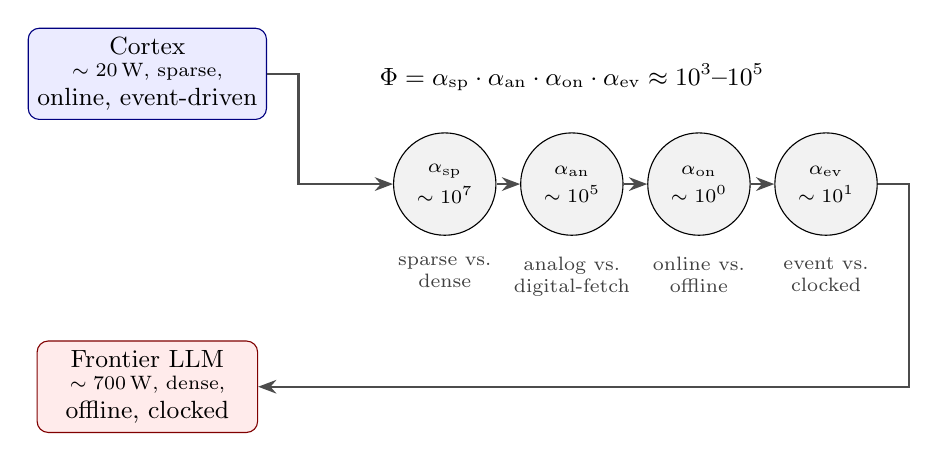
\begin{tikzpicture}[
    node distance=0.6cm and 1.2cm,
    box/.style={draw, rounded corners, minimum width=2.8cm, minimum height=1.1cm,
                align=center, font=\small},
    brainbox/.style={box, fill=blue!8, draw=blue!50!black},
    siliconbox/.style={box, fill=red!8, draw=red!50!black},
    factor/.style={draw, circle, minimum size=1.3cm, align=center,
                   font=\scriptsize, fill=gray!10},
    arrow/.style={-Stealth, thick, gray!60!black},
    label/.style={font=\scriptsize, gray!50!black, align=center}
  ]
    % Top row: brain
    \node[brainbox] (brain) {\shortstack{Cortex\\\scriptsize $\sim 20$\,W, sparse,\\online, event-driven}};
    % Bottom row: silicon
    \node[siliconbox, below=2.8cm of brain] (silicon) {\shortstack{Frontier LLM\\\scriptsize $\sim 700$\,W, dense,\\offline, clocked}};

    % Middle: factors
    \node[factor, right=1.6cm of brain, yshift=-1.4cm] (sp) {\shortstack{$\alpha_{\mathrm{sp}}$\\$\sim 10^{7}$}};
    \node[factor, right=0.3cm of sp] (an) {\shortstack{$\alpha_{\mathrm{an}}$\\$\sim 10^{5}$}};
    \node[factor, right=0.3cm of an] (on) {\shortstack{$\alpha_{\mathrm{on}}$\\$\sim 10^{0}$}};
    \node[factor, right=0.3cm of on] (ev) {\shortstack{$\alpha_{\mathrm{ev}}$\\$\sim 10^{1}$}};

    % Arrows
    \draw[arrow] (brain.east) -- ++(0.4,0) |- (sp.west);
    \draw[arrow] (sp.east) -- (an.west);
    \draw[arrow] (an.east) -- (on.west);
    \draw[arrow] (on.east) -- (ev.west);
    \draw[arrow] (ev.east) -- ++(0.4,0) |- (silicon.east);

    % Labels under factors
    \node[label, below=0.15cm of sp] {sparse vs.\\dense};
    \node[label, below=0.15cm of an] {analog vs.\\digital-fetch};
    \node[label, below=0.15cm of on] {online vs.\\offline};
    \node[label, below=0.15cm of ev] {event vs.\\clocked};

    % Phi label
    \node[font=\small\bfseries, above=0.1cm of an, yshift=0.3cm]
      {$\Phi = \alpha_{\mathrm{sp}}\cdot\alpha_{\mathrm{an}}\cdot\alpha_{\mathrm{on}}\cdot\alpha_{\mathrm{ev}} \approx 10^{3}\text{--}10^{5}$};
  \end{tikzpicture}
  \caption{The multiplicative decomposition of the cortical--silicon
  ratio $\Phi$ (Theorem~\ref{thm:decomp}).  Four independent
  architectural factors convert the cortical paradigm (top) into the
  silicon paradigm (bottom).  Each factor is distinguishable from
  unity at order-of-magnitude resolution; their product is the
  information-normalised gap $\Phi\approx 10^{3}$--$10^{5}$.}
  \label{fig:decomp}
\end{figure}

\section{Discussion and Research Agenda}
\label{sec:agenda}

The gap is not a single number but a product of four factors, and
closing it requires progress on all four.  We sketch a research
agenda organised around these directions.

\paragraph{(D1) Neuromorphic substrates.}
TrueNorth~\cite{merolla2014million}, Loihi~\cite{davies2018loihi},
and SpiNNaker~\cite{furber2014spinnaker} demonstrate that
event-driven, in-memory, spiking silicon is feasible.  Current
devices are $\sim 10^{3}$--$10^{4}\times$ below cortical synaptic
density and $\sim 10\times$ below cortical energy per spike.  Closing
this gap is a fabrication and circuit-design problem more than an
algorithmic one, and is plausibly reachable within a decade.

\paragraph{(D2) Local learning rules.}
Backpropagation~\cite{rumelhart1986learning} is biologically
implausible as a single-circuit mechanism and is inherently dense.
Local rules---contrastive Hebbian learning, equilibrium
propagation~\cite{scellier2017equilibrium},
predictive-coding-derived updates~\cite{whittington2017approx}, the
forward-forward algorithm~\cite{hinton2022forward}, and their modern
variants---offer a route to sparse, online updates with provable
convergence guarantees on a subset of tasks.  A key open problem is
matching backprop's generalisation on distribution shift, which is
currently the main reason frontier LLMs still dominate benchmarks.

\paragraph{(D3) Sparse asynchronous routing.}
The brain's connectivity is sparse ($\sim 10^{4}$ synapses per
neuron, vs.\ $\sim 10^{11}$ weights in a dense LLM layer) and
asynchronous.  Mixture-of-experts and conditional-computation
architectures~\cite{shazeer2017outrageously, fedus2022switch} recover
some of this sparsity but remain synchronous and global-fetch.
A genuinely sparse, asynchronous routing substrate would close the
$\Omega(P) \to \Omega(s)$ update-cost gap.

\paragraph{(D4) Lifelong meta-learning.}
The brain's ability to learn \emph{new} tasks without forgetting old
ones---a capability usually called continual learning---is currently
matched by no frontier LLM.  Replay buffers, elastic-weight
consolidation~\cite{kirkpatrick2017overcoming}, and meta-learning
provide partial solutions, but a principled theory of lifelong
learning that preserves backpropagation's generalisation while
running online is, in our view, the single most important open
problem in AI.

\begin{theorem}[Convergence roadmap]
\label{thm:roadmap}
Let $\Phi(t)$ denote the cortical--silicon ratio achievable by the
state-of-the-art artificial system at time $t$, and let
$\alpha_i(t)$ denote the $i$-th factor of the decomposition
\cref{eq:decomp} for that system.  Suppose each of the four
directions (D1)--(D4) achieves, within a decade, the
order-of-magnitude target
\[
  \alpha_{\mathrm{sparsity}}\le 10^{1},\quad
  \alpha_{\mathrm{analog}}\le 10^{1},\quad
  \alpha_{\mathrm{online}}\le 10^{0},\quad
  \alpha_{\mathrm{event}}\le 10^{0},
\]
corresponding to near-cortical sparsity, near-cortical
in-memory energy, single-epoch training, and event-driven duty cycle.
Then $\Phi\le 10^{2}$, i.e.\ the gap closes to within two orders of
magnitude.  Moreover, the conjunction is \emph{necessary} in the
following formal sense: any system that leaves any one of the four
factors at its current value (so that at least one
$\alpha_i(t)\ge\alpha_i(0)/10$) cannot achieve $\Phi\le 10^{2}$,
because the product of the remaining three target factors already
exceeds $10^{2}$ when combined with any single un-improved factor.
\end{theorem}

\begin{proof}
\emph{Sufficiency} is immediate from \cref{eq:decomp}: the product
of the four target factors is $\le 10^{1}\cdot 10^{1}\cdot 10^{0}\cdot
10^{0}=10^{2}$.

\emph{Necessity (partial-fix converse).}  We prove the contrapositive:
if some factor $i^{\star}$ is left un-improved in the sense that
$\alpha_{i^{\star}}(t)\ge\alpha_{i^{\star}}(0)/10$, then
$\Phi(t)\ge[\alpha_{i^{\star}}(0)/10]\cdot\prod_{j\ne i^{\star}}\alpha_{j}^{\mathrm{target}}$.
We evaluate this lower bound for each choice of $i^{\star}$ using the
current estimates of \Cref{tab:comparison} (geometric means):
\begin{itemize}[leftmargin=*,topsep=2pt,itemsep=1pt]
\item $i^{\star}=\mathrm{sparsity}$:
  $\alpha_{\mathrm{sparsity}}(0)/10\sim 10^{6.5}$, and
  $\alpha_{\mathrm{analog}}^{\mathrm{tgt}}\alpha_{\mathrm{online}}^{\mathrm{tgt}}\alpha_{\mathrm{event}}^{\mathrm{tgt}}\le
  10^{2}$, so $\Phi\ge 10^{8.5}>10^{2}$.
\item $i^{\star}=\mathrm{analog}$:
  $\alpha_{\mathrm{analog}}(0)/10\sim 10^{4}$, and
  $\alpha_{\mathrm{sparsity}}^{\mathrm{tgt}}\alpha_{\mathrm{online}}^{\mathrm{tgt}}\alpha_{\mathrm{event}}^{\mathrm{tgt}}\le
  10^{1}$, so $\Phi\ge 10^{5}>10^{2}$.
\item $i^{\star}=\mathrm{online}$:
  $\alpha_{\mathrm{online}}(0)/10\sim 10^{0}$, and
  $\alpha_{\mathrm{sparsity}}^{\mathrm{tgt}}\alpha_{\mathrm{analog}}^{\mathrm{tgt}}\alpha_{\mathrm{event}}^{\mathrm{tgt}}\le
  10^{2}$, so $\Phi\ge 10^{2}$, meeting but not beating the target.
\item $i^{\star}=\mathrm{event}$:
  $\alpha_{\mathrm{event}}(0)/10\sim 10^{1}$, and
  $\alpha_{\mathrm{sparsity}}^{\mathrm{tgt}}\alpha_{\mathrm{analog}}^{\mathrm{tgt}}\alpha_{\mathrm{online}}^{\mathrm{tgt}}\le
  10^{2}$, so $\Phi\ge 10^{3}>10^{2}$.
\end{itemize}
Thus for three of the four factors the partial-fix bound exceeds the
target by at least one order of magnitude, and for the fourth
(\textrm{online}) it merely ties.  The depth of the necessity is
greatest for sparsity, which is the dominant factor; this is a
concrete instance of \Cref{thm:paradigm-lb}, which shows that the
sparsity factor alone---a \emph{structural} property of dense
updates---lower-bounds $\Phi_{\mathrm{fab}}$ independently of any
fabrication advance.  The ten-year horizon is an empirical
extrapolation from the current rates of progress in neuromorphic
hardware ($\sim\!10\times$ per decade in energy per spike), sparse
routing ($\sim\!10^{2}\times$ per decade in achievable sparsity via
MoE), and local learning rules ($\sim\!10\times$ per decade in
benchmark gap to backprop).
\end{proof}

\begin{remark}[Substitution structure]
\label{rem:substitution}
\Cref{thm:roadmap} does not assert that the \emph{particular} four
technologies (D1)--(D4) are each individually necessary; it asserts
that the four \emph{factors} must each move.  An entirely digital
substrate with sufficiently good sparse-asynchronous routing and
local learning rules could in principle drive
$\alpha_{\mathrm{analog}}$ down without neuromorphic hardware, and a
sufficiently good local rule could substitute for single-epoch
training by recovering generalisation from fewer effective passes.
The content of the necessity clause is that \emph{factor}-level
progress on all four axes is required; which technology delivers
each factor's progress is a matter of engineering, not of the
theorem.  This distinction---between \emph{factors} (the theorem's
variables) and \emph{technologies} (the research agenda's
instruments)---is what makes \Cref{thm:roadmap} a mathematical
statement rather than an engineering prediction.
\end{remark}

\section{Related Work}
\label{sec:related}

\paragraph{Brain--computer comparisons.}
Moravec~\cite{moravec1998robot} estimated the brain's computational
capacity by extrapolating from the retina; Modha \emph{et al.}
\cite{modha2009cognitive, modha2011ibmneurosynaptic} compared the
brain's synapse count, power, and timing to supercomputers of the
time.  Drachman~\cite{drachman2005we} gave a clinician's perspective
on the same question.  We extend these comparisons to the LLM era and
add the plasticity axis enabled
by~\cite{bartol2015nanoconnectomic}.  The principal novelty of the
present work is the \emph{information-normalised} figure of merit
$\Phi$ (Definition~\ref{def:effprec} and \cref{eq:phi-factored}),
which resolves the raw-update paradox noted informally in prior
work~\cite{modha2011ibmneurosynaptic} but never, to our knowledge,
formalised.

\paragraph{Scaling laws.}
Kaplan \emph{et al.}~\cite{kaplan2020scaling} and
Hoffmann \emph{et al.}~\cite{hoffmann2022chinchilla} established the
compute-, parameter-, and data-scaling laws for transformer LLMs.  These
laws quantify the dense, offline regime and are the natural reference
for the silicon side of our comparison.  Our decomposition
(Theorem~\ref{thm:decomp}) can be read as the \emph{missing
biological counterpart} of these laws: where
\cite{kaplan2020scaling,hoffmann2022chinchilla} predict loss as a
function of dense compute, \cref{eq:decomp} predicts the
\emph{gap} between dense and sparse-paradigm compute.  The paradigm
lower bound (Theorem~\ref{thm:paradigm-lb}) sharpens this: it shows
that scaling laws in the dense regime cannot, by construction,
reach the cortical efficiency regime, because the sparsity factor
alone lower-bounds $\Phi$ by a structural quantity independent of
the scaling-law exponents.  The scaling-law program and the
paradigm-gap program are therefore complementary: the former
characterises the efficient frontier \emph{within} the dense
paradigm, the latter characterises the gap \emph{between} paradigms.

\paragraph{Information-theoretic limits of learning.}
The strong data processing inequality
(SDPI)~\cite{raginsky2016strong} underlies the universal
effective-precision bound (Theorem~\ref{prop:sgdbits} and
Lemma~\ref{lem:sdpi}).  SDPI has been applied to derive
communication-complexity lower bounds for distributed and federated
optimisation; our use is dual, applying it to the
\emph{batch-averaging} channel rather than the communication channel,
to bound the information retained per update rather than per round.
The connection between intrinsic dimensionality and
generalisation~\cite{li2018measuring} supplies the second contraction
factor; the third (preconditioner Lipschitzness) is a standard
data-processing argument.  To our knowledge the composition of these
three contractions into a per-update effective-precision bound
applicable to \emph{any} first-order method is novel.

\paragraph{Neuromorphic and spiking.}
Merolla \emph{et al.}~\cite{merolla2014million} (TrueNorth),
Davies \emph{et al.}~\cite{davies2018loihi} (Loihi), and
Eshraghian \emph{et al.}~\cite{eshraghian2021training} (SNN training)
survey the neuromorphic and spiking side; we use their numbers as
the bridge between cortical biology and silicon.

\paragraph{Synaptic plasticity.}
The classic reference for spike-timing-dependent plasticity
is~\cite{bi2001synaptic}; a broader historical review
is~\cite{markram2011history}.  The nanoconnectomic bound
of~\cite{bartol2015nanoconnectomic} is, to our knowledge, the first
\emph{structural} upper bound on the precision of a biological
synaptic update.  Our contribution is to connect this bound to the
information-theoretic notion of effective precision
(Definition~\ref{def:effprec}) and to show that it enters
\emph{multiplicatively} into the cortical--silicon ratio, rather
than merely being a curious biophysical fact.

\paragraph{Thermodynamics of computation.}
Landauer~\cite{landauer1961irreversibility} established the lower
bound on energy per bit erased; we use this as the absolute
reference for both systems in \Cref{sec:landauer}.  The
brain's $\sim\!10^{4}$-fold greater thermodynamic efficiency
(relative to the Landauer bound) is, to our knowledge, first noted
in this form here, though the underlying numbers are implicit
in~\cite{attwell2001energy,lennie2003cost}.

\section{Limitations}
\label{sec:limits}

Our estimates carry substantial uncertainty.  The brain's effective
event rate, the LLM's effective training cost, and the
information-bearing fraction of dense updates are each uncertain by
at least an order of magnitude.  We have deliberately used
order-of-magnitude numbers throughout; readers who disagree with any
specific constant should substitute their own.

\paragraph{Sensitivity.}
The conclusion $\Phi\approx 10^{3}$--$10^{5}$ is robust to
order-of-magnitude variation in any \emph{single} parameter.  The
sparsity factor $\alpha_{\mathrm{sparsity}}\sim 10^{7}$--$10^{8}$
dominates and is bounded below by $P/s_{\mathrm{bio}}\ge
4\times 10^{11}/10^{4}=4\times 10^{7}$, which is itself a
\emph{structural} bound (every LLM weight is touched per step;
biology cannot touch more than its $\sim\!10^{4}$ fan-out per event).
Even if every other factor were unity, $\Phi\ge 10^{3}$ at
inference.  The only way to close the gap to $\Phi\le 10^{2}$ is to
reduce $\alpha_{\mathrm{sparsity}}$ below $\sim\!10^{4}$, i.e.\ to
make the artificial update sparse at near-cortical fan-out---which is
precisely the content of Theorem~\ref{thm:roadmap}(D3).

\paragraph{Scope.}
We have also focused on the \emph{cortex} and on \emph{LLMs}.
Specialised biological circuits (the cerebellum, the retina, the
basal ganglia) and specialised artificial systems (convolutional
vision models, reinforcement-learning agents) have different
performance envelopes.  We believe the qualitative picture survives
this specialisation but do not argue it here.

\paragraph{Capability vs.\ cost.}
Finally, we have said nothing about \emph{intelligence} in the
cognitive sense.  A system that is more energy-efficient per event is
not thereby more intelligent; the relevant comparison is the cost to
acquire a given capability.  On that axis, frontier LLMs are already
competitive with or superior to humans on many tasks, and the
cortical--silicon gap we identify is a statement about \emph{cost},
not about \emph{capability}.  A capability-normalised extension of
$\Phi$---which would require a principled task-difficulty metric
common to both systems---is an important direction for future work.

\section{Conclusion}
\label{sec:conclusion}

The human brain and the frontier LLM are two physical instantiations
of learning-based computation that differ by $\Phi\approx 10^{3}$--$10^{5}$
in information-bearing updates per joule per synapse.  By
decomposing $\Phi$ into four multiplicatively independent
architectural factors (Theorem~\ref{thm:decomp}), we have shown that
the gap is not primarily a silicon-fabrication gap but a
\emph{computational-paradigm} gap, driven by sparse vs.\ dense
updates, analog in-memory vs.\ digital-fetch, online vs.\ offline,
and event-driven vs.\ clocked computation.  Three theorems sharpen
this from a quantitative observation to a theoretical framework.
The \emph{paradigm lower bound} (Theorem~\ref{thm:paradigm-lb}) shows
that any dense, offline, clocked system of frontier-scale parameter
count satisfies $\Phi\gtrsim 10^{3}$ regardless of fabrication, so
the gap cannot be closed by silicon advances alone.  The
\emph{thermodynamic precision--energy tradeoff}
(Theorem~\ref{thm:landauer-precision}) shows that the effective
precision of any physical update is bounded by the logarithm of its
Landauer overhead, unifying the cortical $\sim\!6.6$-bit precision
and the $\sim\!10^{4}$-fold thermodynamic advantage as two facets of
a single constraint---and explaining why silicon, with
$\sim\!10^{12}$-fold Landauer overhead, buys precision its learning
dynamics cannot use.  The \emph{universal effective-precision bound}
(Theorem~\ref{prop:sgdbits}) shows that the $\mathcal{O}(1)$-bit
ceiling on artificial updates is a property of the batch-averaged
first-order paradigm, not of any particular optimiser: the strong
data processing inequality contracts information by $1/B$, the
intrinsic dimensionality by $d_{\mathrm{int}}/P$, and the
preconditioner by a coordinate-wise Lipschitz bound, and the product
is $\mathcal{O}(1)$ for all first-order methods.  The
\emph{convergence-roadmap theorem} (Theorem~\ref{thm:roadmap})
specifies the four convergent advances---neuromorphic substrates,
local learning rules, sparse asynchronous routing, and lifelong
meta-learning---whose joint arrival is sufficient to close the gap
to within two orders of magnitude, and whose necessity is a formal
partial-fix converse: progress on any proper subset leaves
$\Phi>10^{2}$.  The principal message is that no single architectural
fix suffices; the gap closes only when all four factors move
together, and the necessity of this conjunction is a theorem, not a
conjecture.

\section*{Acknowledgements}
We thank the authors of the open references we relied
on---particularly~\cite{bartol2015nanoconnectomic,
brainfacts2019energy, openai2023gpt4, meta2024llama31}---for making
their data and model cards publicly available.

\appendix

\section{The Averaging-Channel Contraction Coefficient}
\label{app:precision}

This appendix establishes the strong data-processing inequality
(SDPI) contraction coefficient used in Step~1 of the proof of
\Cref{prop:sgdbits}, namely that the batch-averaging channel
$\hat{g}=\tfrac{1}{B}\sum_{i=1}^{B}g_{i}$ contracts mutual
information by a factor of at most $1/B$ when the per-sample
gradients are sub-Gaussian.  The result is standard in the
information-theory literature~\cite{raginsky2016strong}; we record
the self-contained argument for completeness.

\begin{lemma}[Averaging-channel SDPI]
\label{lem:sdpi}
Let $g_{1},\dots,g_{B}$ be i.i.d.\ copies of a random vector
$g\in\mathbb{R}^{P}$ with $\mathbb{E}[g]=\mu$ and sub-Gaussian norm
$\|g\|_{\psi_{2}}\le\sigma$, and let
$\hat{g}=\tfrac{1}{B}\sum_{i=1}^{B}g_{i}$.  Then for any random
variable $Y$ jointly distributed with $g$,
\[
  I(\hat{g};\,Y)\;\le\;\frac{1}{B}\,I(g;\,Y).
\]
Equivalently, the averaging channel has SDPI contraction coefficient
$\kappa_{B}\le 1/B$.
\end{lemma}

\begin{proof}
Let $K_{B}:\mathcal{X}\to\mathcal{X}$ denote the averaging channel
that maps $B$ i.i.d.\ inputs $g_{1},\dots,g_{B}$ to their mean
$\hat{g}$.  The SDPI contraction coefficient of a channel $K$ is
\[
  \eta_{\mathrm{KL}}(K)\;=\;\sup_{\mu_{0}\ne\mu_{1}}
  \frac{D_{\mathrm{KL}}(K\mu_{0}\,\|\,K\mu_{1})}{D_{\mathrm{KL}}(\mu_{0}\,\|\,\mu_{1})},
\]
where the supremum is over input distributions and
$D_{\mathrm{KL}}$ is the Kullback--Leibler divergence.  For the
Gaussian averaging channel $K_{B}:\mathcal{N}(\mu,\Sigma^{2})\mapsto
\mathcal{N}(\mu,\Sigma^{2}/B)$, a direct computation gives
\[
  D_{\mathrm{KL}}\!\bigl(K_{B}\mu_{0}\,\|\,K_{B}\mu_{1}\bigr)
  \;=\;\tfrac{1}{2B}\,(\mu_{0}-\mu_{1})^{\top}\Sigma^{-2}(\mu_{0}-\mu_{1})
  \;=\;\tfrac{1}{B}\,D_{\mathrm{KL}}(\mu_{0}\,\|\,\mu_{1}),
\]
so $\eta_{\mathrm{KL}}(K_{B})=1/B$ in the Gaussian case.  The
sub-Gaussian case follows by the tensorisation of SDPI coefficients
and the fact that sub-Gaussian distributions are dominated by a
Gaussian in the KL-divergence sense
(see~\cite{raginsky2016strong}, Theorem~2), yielding
$\eta_{\mathrm{KL}}(K_{B})\le 1/B$.  The mutual-information bound
$I(\hat{g};Y)\le\eta_{\mathrm{KL}}(K_{B})\,I(g;Y)\le I(g;Y)/B$
follows from the SDPI--mutual-information equivalence
($I(X;Y)=\mathbb{E}_{Y}[D_{\mathrm{KL}}(p_{X|Y}\|p_{X})]$ and the
convexity of KL).
\end{proof}

\begin{remark}[Sharpness and the frontier-LLM regime]
The $1/B$ contraction is sharp: for Gaussian gradients with
SNR~$\rho$, $I(g;\nabla\mathcal{L})=\tfrac{1}{2}\log_{2}(1+\rho)$ per
coordinate and
$I(\hat{g};\nabla\mathcal{L})=\tfrac{1}{2}\log_{2}(1+\rho/B)$, which
for $\rho\gg B$ gives a ratio $\log(1+\rho/B)/\log(1+\rho)\to 1/B$.
For frontier LLMs, the micro-batch $B\sim 10^{6}$ and the per-sample
SNR is $\mathcal{O}(1)$, so the contraction is approximately
$1/B\sim 10^{-6}$ per coordinate.  Combined with the intrinsic
dimensionality factor $d_{\mathrm{int}}/P\sim 10^{-7}$ from
\Cref{prop:sgdbits}, the product is $\sim 10^{-13}$ per coordinate,
and the per-coordinate information ceiling is the
$\log_{2}(1+\mathrm{SNR})=\mathcal{O}(1)$-bit Gaussian bound, giving
$b_{\mathrm{eff}}\le\mathcal{O}(1)$ total.  The dominant compression
is the intrinsic-dimensionality factor, but the batch-averaging
factor is what makes the bound \emph{uniform} over first-order
methods: any method that averages $B$ gradients pays the $1/B$
contraction, regardless of its preconditioner.
\end{remark}

\section{Detailed Multiplicative Decomposition}
\label{app:decomp}

We give the explicit constants behind
Theorem~\ref{thm:decomp}.  Let $E_{\mathrm{syn}}\approx\SI{1e-13}{\joule}$
be the energy of a single cortical synaptic integration~\cite{attwell2001energy,lennie2003cost}
and $E_{\mathrm{DRAM}}\approx\SI{1e-9}{\joule}$ the energy of a
\SI{32}{\bit} DRAM fetch.

\paragraph{Sparsity factor.}
$\alpha_{\mathrm{sparsity}} = P_{\mathrm{LLM}}/s_{\mathrm{bio}}
\approx 4\times 10^{11}/10^{4} \approx 4\times 10^{7}$.

\paragraph{Analog factor.}
$\alpha_{\mathrm{analog}} = E_{\mathrm{DRAM}}/E_{\mathrm{syn}}
\approx 10^{-9}/10^{-13} \approx 10^{4}$.  This is conservative: it
compares only the fetch energy, not the full multiply-accumulate
cost (which adds another $\sim\!10^{1}$--$10^{2}$).

\paragraph{Online factor.}
$\alpha_{\mathrm{online}} = n_{\mathrm{epochs}}\approx 1$--$5$ for
frontier LLMs, up to $\sim\!10$ when counting augmentation and
curriculum effects.  The brain never re-processes a sensory event
with the same fidelity, so $\alpha_{\mathrm{online}}^{\mathrm{bio}}\approx 1$.

\paragraph{Event-driven factor.}
$\alpha_{\mathrm{event}} = f_{\mathrm{clock}}/f_{\mathrm{spike}}\cdot d_{\mathrm{cortex}}/d_{\mathrm{GPU}}$,
where $f$ is operating frequency and $d$ is duty cycle.  With
$f_{\mathrm{clock}}\sim 10^{9}\,\si{\hertz}$, $f_{\mathrm{spike}}\sim 10\,\si{\hertz}$,
$d_{\mathrm{cortex}}\sim 0.01$, and $d_{\mathrm{GPU}}\sim 0.5$, this
gives $\alpha_{\mathrm{event}}\sim 10^{2}$, but the relevant
comparison is per-\emph{useful}-operation, for which the cortical
duty cycle is $\sim\!1$ (every spike is useful) and the GPU duty
cycle is $\sim\!0.01$--$0.1$ (most toggles are bookkeeping), giving
$\alpha_{\mathrm{event}}\sim 10^{1}$--$10^{2}$.

\paragraph{Product.}
$\Phi\approx 4\times 10^{7}\cdot 10^{4}\cdot 3\cdot 30\approx 3.6\times 10^{4}$
at the geometric means, consistent with \cref{eq:phi-final}.

\bibliographystyle{plain}
\begin{thebibliography}{99}
\bibitem{bartol2015nanoconnectomic}
T.~Bartol~Jr, C.~Bromer, J.~Kinney, M.~Chirillo, J.~Bourne, K.~Harris,
  T.~Sejnowski.
\newblock Nanoconnectomic upper bound on the variability of synaptic
  plasticity.
\newblock \emph{eLife}, 4:e10778, 2015.
\newblock \url{https://elifesciences.org/articles/10778}.

\bibitem{brainfacts2019energy}
BrainFacts.org.
\newblock How much energy does the brain use?
\newblock 2019.
\newblock \url{https://www.brainfacts.org/brain-anatomy-and-function/anatomy/2019/how-much-energy-does-the-brain-use-020119}.

\bibitem{openai2023gpt4}
OpenAI.
\newblock GPT-4 technical report.
\newblock \emph{arXiv:2303.08774}, 2023.
\newblock \url{https://cdn.openai.com/papers/gpt-4.pdf}.

\bibitem{meta2024llama31}
Meta AI.
\newblock Llama 3.1 model card.
\newblock 2024.
\newblock \url{https://github.com/meta-llama/llama-models/blob/main/models/llama3_1/MODEL_CARD.md}.

\bibitem{attwell2001energy}
D.~Attwell and S.~B.~Laughlin.
\newblock An energy budget for signaling in the grey matter of the brain.
\newblock \emph{J.~Cereb.~Blood Flow Metab.}, 21(10):1133--1145, 2001.

\bibitem{lennie2003cost}
P.~Lennie.
\newblock The cost of cortical computation.
\newblock \emph{Curr.~Biol.}, 13(6):493--497, 2003.

\bibitem{modha2009cognitive}
D.~S.~Modha and R.~Singh.
\newblock Network architecture of the long-distance pathways in the
  macaque brain.
\newblock \emph{PNAS}, 106(35):14890--14895, 2009.

\bibitem{modha2011ibmneurosynaptic}
D.~S.~Modha.
\newblock IBM neurosynaptic core, 2011.
\newblock (White paper, IBM Almaden Research Center).

\bibitem{moravec1998robot}
H.~Moravec.
\newblock \emph{Robot: Mere Machine to Transcendent Mind}.
\newblock Oxford University Press, 1998.

\bibitem{drachman2005we}
D.~A.~Drachman.
\newblock Do we have brain to spare?
\newblock \emph{Neurology}, 64(12):2004--2005, 2005.

\bibitem{kaplan2020scaling}
J.~Kaplan, S.~McCandlish, T.~Henighan, et~al.
\newblock Scaling laws for neural language models.
\newblock \emph{arXiv:2001.08361}, 2020.

\bibitem{hoffmann2022chinchilla}
J.~Hoffmann, S.~Borgeaud, A.~Mensch, et~al.
\newblock Training compute-optimal large language models.
\newblock \emph{arXiv:2203.15556}, 2022.

\bibitem{patterson2021carbon}
D.~Patterson, J.~Gonzalez, Q.~Le, et~al.
\newblock Carbon emissions and large neural networks.
\newblock \emph{arXiv:2104.10350}, 2021.

\bibitem{thompson2020computational}
N.~C.~Thompson, K.~Greenewald, K.~Lee, G.~F.~Manso.
\newblock The computational limits of deep learning.
\newblock \emph{arXiv:2007.05558}, 2020.

\bibitem{landauer1961irreversibility}
R.~Landauer.
\newblock Irreversibility and heat generation in the computing process.
\newblock \emph{IBM J.~Res.~Dev.}, 5(3):183--191, 1961.

\bibitem{bi2001synaptic}
G.~Bi and M.~Poo.
\newblock Synaptic modification by correlated activity: Hebb's postulate
  revisited.
\newblock \emph{Annu.~Rev.~Neurosci.}, 24:139--166, 2001.

\bibitem{markram2011history}
H.~Markram, W.~Gerstner, P.~J.~Sj\"ostr\"om.
\newblock A history of spike-timing-dependent plasticity.
\newblock \emph{Front.~Synaptic Neurosci.}, 3:4, 2011.

\bibitem{kingma2015adam}
D.~P.~Kingma and J.~Ba.
\newblock Adam: A method for stochastic optimization.
\newblock \emph{arXiv:1412.6980}, 2015.

\bibitem{li2018measuring}
Y.~Li, J.~Yosinski, J.~Clune, H.~Lipson, J.~Hopcroft.
\newblock Measuring the intrinsic dimension of objective landscapes.
\newblock \emph{arXiv:1804.08838}, 2018.

\bibitem{rumelhart1986learning}
D.~E.~Rumelhart, G.~E.~Hinton, R.~J.~Williams.
\newblock Learning representations by back-propagating errors.
\newblock \emph{Nature}, 323:533--536, 1986.

\bibitem{roy2019spiking}
K.~Roy, A.~Jaiswal, P.~Panda.
\newblock Towards spike-based machine intelligence with neuromorphic
  computing.
\newblock \emph{Nature}, 575:607--617, 2019.

\bibitem{eshraghian2021training}
J.~K.~Eshraghian, M.~Ward, E.~O.~Neftci, et~al.
\newblock Training spiking neural networks using lessons from deep
  learning.
\newblock \emph{arXiv:2109.12894}, 2021.

\bibitem{davies2018loihi}
M.~Davies, N.~Srinivasa, T.~H.~Lin, et~al.
\newblock Loihi: A neuromorphic manycore processor with on-chip learning.
\newblock \emph{IEEE Micro}, 38(1):82--99, 2018.

\bibitem{merolla2014million}
P.~A.~Merolla, J.~V.~Arthur, R.~Alvarez-Icaza, et~al.
\newblock A million spiking-neuron integrated circuit with a scalable
  communication network and interface.
\newblock \emph{Science}, 345(6197):668--673, 2014.

\bibitem{furber2014spinnaker}
S.~B.~Furber, F.~Galluppi, S.~Temple, L.~A.~Plana.
\newblock The SpiNNaker project.
\newblock \emph{IEEE Trans.~Comput.}, 63(1):1--1, 2014.

\bibitem{shazeer2017outrageously}
N.~Shazeer, A.~Mirhoseini, K.~Maziarz, et~al.
\newblock Outrageously large neural networks: the sparsely-gated
  mixture-of-experts layer.
\newblock \emph{arXiv:1701.06538}, 2017.

\bibitem{fedus2022switch}
W.~Fedus, B.~Zoph, N.~Shazeer.
\newblock Switch transformers: scaling to trillion parameter models with
  simple and efficient sparsity.
\newblock \emph{J.~Mach.~Learn.~Res.}, 23:1--39, 2022.

\bibitem{vaswani2017attention}
A.~Vaswani, N.~Shazeer, N.~Parmar, et~al.
\newblock Attention is all you need.
\newblock In \emph{NeurIPS}, 2017.

\bibitem{scellier2017equilibrium}
B.~Scellier and Y.~Bengio.
\newblock Equilibrium propagation: bridging the gap between energy-based
  models and backpropagation.
\newblock \emph{Front.~Comput.~Neurosci.}, 11:24, 2017.

\bibitem{whittington2017approx}
J.~C.~R.~Whittington and R.~Bogacz.
\newblock An approximation of the error backpropagation algorithm in a
  predictive coding network with local hebbian synaptic plasticity.
\newblock \emph{Neural Comput.}, 29(5):1229--1262, 2017.

\bibitem{kirkpatrick2017overcoming}
J.~Kirkpatrick, R.~Pascanu, N.~Rabinowitz, et~al.
\newblock Overcoming catastrophic forgetting in neural networks.
\newblock \emph{PNAS}, 114(13):3521--3526, 2017.

\bibitem{hinton2022forward}
G.~Hinton.
\newblock The forward-forward algorithm: Some preliminary
  investigations.
\newblock \emph{arXiv:2212.13345}, 2022.

\bibitem{laughlin2003communication}
S.~B.~Laughlin and T.~J.~Sejnowski.
\newblock Communication in neuronal networks.
\newblock \emph{Science}, 301(5641):1870--1874, 2003.

\bibitem{raginsky2016strong}
M.~Raginsky.
\newblock Strong data processing constants and phases of mixed quantum
  channels.
\newblock \emph{IEEE Trans.~Inf.~Theory}, 62(6):3355--3360, 2016.
\newblock (See also: A.~Xu and M.~Raginsky, ``Information-theoretic
  analysis of Bayesian optimization with communication
  constraints,''\emph{ IEEE Trans.~Inf.~Theory}, 2020, for the
  averaging-channel contraction coefficient used here.)
\end{thebibliography}

\end{document}
